% !TeX program = pdflatex

\documentclass{article}
\usepackage [utf8] {inputenc} 

\usepackage{graphicx}
\usepackage{siunitx}
\usepackage{longtable}
\usepackage{booktabs}
\usepackage{float}
\usepackage{hyperref}
\usepackage{amsmath}

\usepackage[a4paper, total={6in, 8in}]{geometry}

\usepackage[toc,acronym]{glossaries}
\loadglsentries{glossary}
\makeglossaries

\usepackage[
backend=bibtex,
style=alphabetic,
sorting=ynt
]{biblatex}
\bibliography{bibliography.bib}


\providecommand{\tightlist}{%s
	\setlength{\itemsep}{0pt}\setlength{\parskip}{0pt}}

\title{Experiment Report: \\
	"Performance Analysis Framework For Base Station Placement Using IEEE 802.11"
}
\author{Kukartsev Kirill,Rustam Khakov, Zufar Makhmutov }

\begin{document}
	
	\maketitle
	
	\clearpage
	
	\tableofcontents
	\newpage
	
	\section{Formal Description of the
experiment}\label{formal-description-of-the-experiment}

In the experiment we seek to:

\begin{enumerate}
\def\labelenumi{\arabic{enumi}.}
\tightlist
\item
  Check the functionality of experimental software system.
  
  \begin{itemize}
  	\tightlist
  	\item
  	Check the functional properties of the system.
  	\item
  	Stability, performance and usability of the components in real case
  	scenarios.
  \end{itemize}

\item
  Evaluation of \gls{unmanned_aerial_vehicle}s (having Wi-Fi \gls{access_point}) layout
  optimization algorithms.
  
  \begin{itemize}
  	\tightlist
  	\item
  	Evaluation of correctness of provided optimized positions by the
  	algorithms.
  	\item
  	Measurement of stability, performance, and usability of the
  	algorithms.
  \end{itemize}
  
\end{enumerate}


\subsection{Main information}\label{main-information}

The main purpose of the experiment is to optimize the location of \gls{access_point}'s in 
a such way that throughput and RSS of UE's connected to those AP is
maximized.

For that we experiment with the following way:

\begin{enumerate}
\def\labelenumi{\arabic{enumi}.}
\tightlist
\item
  APs located in the space without any obstacles. They are surrounded by
  UEs.
\item
  UEs connected to APs and evaluate RSS and throughput via specially
  designed software.
\item
  Stored measured records by UEs are sent/copied to the central server.
\item
  An operator uses the provided interface to analyze the measurements
  and run optimization algorithms to find out the best positions for
  APs.
\item
  After the next optimal positions for APs are found, access points
  moved to the optimized points.
\item
  An experiment is going to step 3 and repeated until no significant
  improvement for APs positions will be observed.
\end{enumerate}

The experiment repeated three times with different initial APs and UE
positions.

Test sets:

\begin{enumerate}
\def\labelenumi{\arabic{enumi}.}
\tightlist
\item
  Suboptimal (APs in between clusters)
\item
  Near-optimal (APs in clusters according to K-Means.)
\item
  Uniform (in the area)
\end{enumerate}

For each test case, we expect that:

\begin{enumerate}
\def\labelenumi{\arabic{enumi}.}
\tightlist
\item
  Minimization of the distance between UEs and APs will lead to RSS gain
  and throughput increase.
\item
  The interference effect may be visible -- in the suboptimal
  placements, it should decrease the throughput;
\end{enumerate}
	\section{Experiment requirement}\label{experiment-requirement}

\subsection{Hardware Equipment}\label{hardware-equipment}

\begin{itemize}
\tightlist
\item
  6 cellphones with Android \acrshort{os} (version 5.0 and above). A dedicated \gls{gnss}
  and \gls{wifi} modules.
\item
  3 external \gls{wifi} Adapters with managed mode.

  \begin{itemize}
  \tightlist
  \item
    Model: AWUS036NEH
  \item
    Antenna's height for \gls{command_n_center}: 17.2 cm
  \item
    Antenna's height for \gls{access_point}: 11 cm
  \end{itemize}
\item
  3 Laptops.
\item
  One ruler.
\item
  Optionally, means against extreme temperatures, humidity, and so on.
\end{itemize}

\subsection{Software Equipment}\label{software-equipment}

\subsubsection{For \glsentrytext{ue} }

\begin{itemize}
\tightlist
\item
  Android-enabled smartphone (version 5.0 and above).

  \begin{itemize}
  \tightlist
  \item
  	\Gls{gps_android} installed.
    \end{itemize}
\end{itemize}

\subsubsection{For \glsentrytext{command_n_center} }\label{for-command-center-cnc}

\begin{itemize}
\tightlist
\item
  The host machine

\begin{itemize}
	\tightlist
	\item
	Any Debian-based \acrshort{os} (Debian, Ubuntu, etc.).
	\item
	\gls{virtualbox} + \gls{virtualbox_ext_pack} latest version.
	\item
	\gls{python3} + \gls{ansible} (for convenient configuration) installed.
	\item
	\texttt{openssh-server}.
\end{itemize}
\item
  The virtual \gls{command_n_center} machine

  \begin{itemize}
  \tightlist
  \item
    \texttt{dnsmasq}, \texttt{hostapd} installed.
  \item
    \texttt{openssh-server} installed.
  \item
    \texttt{docker} and \texttt{docker-compose} installed.
  \item
  	\texttt{iperf3} installed.

    \begin{itemize}
    \tightlist
    \item
      \gls{mongodb} container.
    \item
      \gls{rabbitmq} container.
    \item
      \gls{mqtt} broker container.
    \item
      \gls{python3} container.
    \item
      \gls{nginx} container.
    \item
      \gls{nodejs} container.
    \end{itemize}
  \end{itemize}
\end{itemize}

\subsubsection{For \glsentrytext{access_point}}\label{for-aps}

\begin{itemize}
\tightlist
\item
The host machine

\begin{itemize}
	\tightlist
	\item
	Any Debian-based \acrshort{os} (Debian, Ubuntu, etc.).
	\item
	\gls{virtualbox} + \gls{virtualbox_ext_pack} latest version.
	\item
	\gls{python3} + \gls{ansible} (for convenient configuration) installed.
	\item
	\texttt{openssh-server}.
\end{itemize}
\item
  The virtual \gls{access_point} machine

  \begin{itemize}
  \tightlist
  \item
    Any Debian-based \acrshort{os} (Debian, Ubuntu, etc.).
  \item
    \texttt{dnsmasq}, \texttt{hostapd} installed.
  \item
    \texttt{iperf3} installed.
  \item
    \texttt{openssh-server} installed.
  \item
    \texttt{docker} and \texttt{docker-compose} installed.

    \begin{itemize}
    \tightlist
    \item
      \acrshort{ftp}-server container.
    \end{itemize}
  \end{itemize}
\end{itemize}

	\section{Experiment preparation procedures}\label{experiment-preparation-procedures}

These steps influence experiment parameters. We aim to take into account
environmental conditions and to minimize noise components.


\subsection{Preparation steps}\label{steps}

\subsubsection{Prepare hardware and software bundles}

Early preparation will solve possible problems during real experiment.

\subsubsection{Install \gls{gps_android} on \glspl{ue}}

Before the experiment, software must be already installed on \gls{android} phones to ensure compatibility.

\subsubsection{Check the weather condition}

Specific environment condition (such as snow or rain) may damage equipment
and disrupt experiment result.

\subsubsection{Check the \gls{rss} attenuation}

This parameter will influence size of area used to place \glspl{ap} and \glspl{ue}.


\subsubsection{Measure the experiment area and place \glspl{ue} on the field}

In case if \gls{rss} is high enough (level of highness evaluated by expert method) there is no reason to use a smaller area
because the radio link quality would remain the same.
	\hypertarget{experiment-description}{%
\section{Experiment description}\label{experiment-description}}

\hypertarget{general-perspective}{%
\subsection{General perspective}\label{general-perspective}}

\begin{figure}[H]
\centering
\includegraphics[width=\linewidth,keepaspectratio]{images/Deployment Diagram-Free-structure_scheme.png}
\caption{Main scenario of the experiment}
\label{fig:experiment-overall-layout}
\end{figure}

From the general system engineering perspective, the experiment is a set
of wireless-connected nodes (via Wi-Fi 802.11n (300 mbps)) which measures the receiving signal strength and measure the throughput of the link to upload and download.

All connections are wireless on each bearer:

\begin{itemize}
\tightlist
\item
  UE \textless{}-\textgreater{} AP.
\item
  AP \textless{}-\textgreater{} CnC.
\end{itemize}

There investigated one problem: the experimental network bandwidth
between UE and AP measurements with \texttt{iperf3} showed about
\textbf{30 MBit/s} speed rate. On the contrary, speed on the bearer UE \textless{}- AP -CnC\textgreater{} showed about \textbf{12-15 MBit/s} speed rate. There is markedly seen a drop in speed rate, probably, because of transmission on the radio channel two-times. The problem  is not in the Wi-Fi itself, but in the fact that radio (wireless) link is not as reliable, as a cord one, so the active bandwidth measurement part must be located as close to the APs as possible - in our case, the server-side \texttt{iperf3} is located in \acrshort{ap}s.

Each UE has two programs on board:

\begin{itemize}
\tightlist
\item
  \texttt{GPS\_Android} - special software designed to perform \acrshort{rss} and  link measurements linked to GPS coordinates.
\item
  \texttt{Magic\ iperf} - a network bandwidth measurement software.  Provides a user-friendly interface to client-side app \texttt{iperf}  on Android phones.
\end{itemize}

Each APs has two Wi-Fi adapters. Since we use laptops to run APs, they expected to have one already included, thus one external extra required for each AP. The internal Wi-Fi adapter connects to the CnC provided Wi-Fi network, the external Wi-Fi adapter creates the access point named
``\textbf{ap}'' for the UEs.

The CnC uses one external AP to create the access point named
``\textbf{cnc}''.

\hypertarget{deployment-diagram}{%
\subsection{Deployment Diagram}\label{deployment-diagram}}

\begin{longtable}[]{@{}ll@{}}
\caption{The main deployed components.}\tabularnewline
\toprule
\begin{minipage}[b]{0.16\columnwidth}\raggedright
Component\strut
\end{minipage} & \begin{minipage}[b]{0.78\columnwidth}\raggedright
Description\strut
\end{minipage}\tabularnewline
\midrule
\endfirsthead
\toprule
\begin{minipage}[b]{0.16\columnwidth}\raggedright
Component\strut
\end{minipage} & \begin{minipage}[b]{0.78\columnwidth}\raggedright
Description\strut
\end{minipage}\tabularnewline
\midrule
\endhead
\begin{minipage}[t]{0.16\columnwidth}\raggedright
Android smartphone group (UEs)\strut
\end{minipage} & \begin{minipage}[t]{0.78\columnwidth}\raggedright
A set of smartphones running Android OS (version 5.0+) with dedicated
Wi-Fi and installed software.\strut
\end{minipage}\tabularnewline
\begin{minipage}[t]{0.16\columnwidth}\raggedright
Access points (APs)\strut
\end{minipage} & \begin{minipage}[t]{0.78\columnwidth}\raggedright
The computers running a Wi-Fi AP software for the UEs connection. Pass
traffic through to CnC and take part in RSS and link quality
measurement.\strut
\end{minipage}\tabularnewline
\begin{minipage}[t]{0.16\columnwidth}\raggedright
Command Center (CnC)\strut
\end{minipage} & \begin{minipage}[t]{0.78\columnwidth}\raggedright
A computing node running the optimization software. Should be provided
with sufficient hardware resources.\strut
\end{minipage}\tabularnewline
\bottomrule
\end{longtable}

From the deployment view, we are using a complicated combination of
software and hardware.

We prefer to run AP and designed software separately in a virtual
machine. That helps to automate development, testing, and maintenance
routines.

\begin{figure}[H]
\centering
\includegraphics[width=\linewidth, keepaspectratio]{images/Deployment Diagram-Deployment_Diagram.png}
\caption{Deployment Diagram}
\label{fig:deployment-diagram}
\end{figure}

\hypertarget{command-center-deployment-cnc}{%
\subsubsection{Command center deployment
(CnC)}\label{command-center-deployment-cnc}}

The CnC software runs on Debian OS in VirtualBox virtual machine.
\texttt{GPS\_Tracker} and \texttt{GPS\_Frontend} are designed to run in
Docker containers. For the experiment, the virtual machine has \textbf{docker}
and \textbf{docker-compose} installed to run these containers. It possible to have performance decrease because of running in containers, however more powerful hardware resources compensates those possible consequences of additional run-time level.

The AP software consists of two packages:

\begin{itemize}
\tightlist
\item
  \texttt{hostapd} - software to manage and run Wi-Fi access points.
\item
  \texttt{dnsmasq} - DNS/DHCP server, to provide an IP address, routing
  and DNS information via DHCP protocol.
\end{itemize}

The AP software starts in the virtual machine, which can access the physical Wi-Fi adapter using the hardware pass-through function from the host machine.

For easy-to-run configuration and deployment of the CnC, there are
provided an \textbf{Ansible} script.

\hypertarget{access-points-deployment-aps}{%
\subsubsection{Access Points deployment
(APs)}\label{access-points-deployment-aps}}

Unlike CnC, physical nodes run the AP software and server-side
\texttt{iperf3} app.

\hypertarget{network-diagram}{%
\subsection{Network Diagram}\label{network-diagram}}

The APs subnet has identical settings. These
\texttt{Wi-Fi\ HotSpot\ Network} has an internal DHCP server to provide
dynamic addresses for connected UEs. To prevent the network IP addresses
collisions and simplify routing, the APs perform masquerading
(SNAT/DNAT) on the output interface (the internal interface used to
connect to CnC). On the one side, it cannot access the UEs directly from
CnC, but the UEs will always reach CnC as long as DHCP sets the default
gateway IP address.

In \texttt{Wi-Fi\ CnC\ Network} installed another DHCP server. It used
to reply to connecting APs with dynamic addresses. Because the subnet
used in this network is different from the internal Wi-Fi adapter's
network in the APs, there is no network collision.

Finally, the UEs can access the static CnC address \texttt{192.168.20.1}
as well as its local AP's gateway address \texttt{192.168.10.1}.


\begin{figure}[H]
	\centering
	\includegraphics[width=\linewidth, keepaspectratio]{images/Deployment Diagram-Network_Diagram.png}
\caption{Network Diagram}
\label{fig:network-diagram}
\end{figure}

\hypertarget{experiment-steps}{%
\subsection{Experiment Steps}\label{experiment-steps}}

The following steps will be executed for each described experimental
case:

\begin{longtable}[]{@{}lll@{}}
\caption{Steps for one experimental case.}\tabularnewline
\toprule
\begin{minipage}[b]{0.01\columnwidth}\raggedright
No\strut
\end{minipage} & \begin{minipage}[b]{0.35\columnwidth}\raggedright
Step\strut
\end{minipage} & \begin{minipage}[b]{0.55\columnwidth}\raggedright
Description\strut
\end{minipage}\tabularnewline
\midrule
\endfirsthead
\toprule
\begin{minipage}[b]{0.01\columnwidth}\raggedright
No\strut
\end{minipage} & \begin{minipage}[b]{0.35\columnwidth}\raggedright
Step\strut
\end{minipage} & \begin{minipage}[b]{0.55\columnwidth}\raggedright
Description\strut
\end{minipage}\tabularnewline
\midrule
\endhead
\begin{minipage}[t]{0.01\columnwidth}\raggedright
1\strut
\end{minipage} & \begin{minipage}[t]{0.35\columnwidth}\raggedright
Initialize network connectivity between APs and CnCs\strut
\end{minipage} & \begin{minipage}[t]{0.55\columnwidth}\raggedright
Ensure that these nodes are available in the network by the ICMP
protocol\strut
\end{minipage}\tabularnewline
\begin{minipage}[t]{0.01\columnwidth}\raggedright
2\strut
\end{minipage} & \begin{minipage}[t]{0.35\columnwidth}\raggedright
Run the software for the experiment\strut
\end{minipage} & \begin{minipage}[t]{0.55\columnwidth}\raggedright
Startup GPS\_Tracker, GPS\_Frontend\strut
\end{minipage}\tabularnewline
\begin{minipage}[t]{0.01\columnwidth}\raggedright
3\strut
\end{minipage} & \begin{minipage}[t]{0.35\columnwidth}\raggedright
Place the APs and UEs according to an experiment case\strut
\end{minipage} & \begin{minipage}[t]{0.55\columnwidth}\raggedright
There are specific predefined positions for each element on the
experiment area.\strut
\end{minipage}\tabularnewline
\begin{minipage}[t]{0.01\columnwidth}\raggedright
4\strut
\end{minipage} & \begin{minipage}[t]{0.35\columnwidth}\raggedright
Measure RSS, Link quality for the initial layout\strut
\end{minipage} & \begin{minipage}[t]{0.55\columnwidth}\raggedright
Measurements are done via GPS\_Android that sends the result to
GPS\_Tracker\strut
\end{minipage}\tabularnewline
\begin{minipage}[t]{0.01\columnwidth}\raggedright
5\strut
\end{minipage} & \begin{minipage}[t]{0.35\columnwidth}\raggedright
Run the APs location optimization for each algorithm in
GPS\_Tracker\strut
\end{minipage} & \begin{minipage}[t]{0.55\columnwidth}\raggedright
Each optimization algorithm can produce different probable positions for
the same UE positions and measurements.\strut
\end{minipage}\tabularnewline
\begin{minipage}[t]{0.01\columnwidth}\raggedright
6\strut
\end{minipage} & \begin{minipage}[t]{0.35\columnwidth}\raggedright
Move the APs to the optimized positions\strut
\end{minipage} & \begin{minipage}[t]{0.55\columnwidth}\raggedright
It is expected that new positions for APs would increase our network
efficiency.\strut
\end{minipage}\tabularnewline
\begin{minipage}[t]{0.01\columnwidth}\raggedright
7\strut
\end{minipage} & \begin{minipage}[t]{0.35\columnwidth}\raggedright
Repeat RSS and Link quality measurements for the optimized APs
positions\strut
\end{minipage} & \begin{minipage}[t]{0.55\columnwidth}\raggedright
1-3 interactions for optimization per each case.\strut
\end{minipage}\tabularnewline
\bottomrule
\end{longtable}

	\section{Near-Optimal layout}\label{near-optimal-layout}

Figure \ref{fig:near-optimal-layout} shows Near-optimal case. Here \glspl{access_point} are placed in the ground
so that both of them are in the center of the corresponding quarter (2nd and 3rd) 25x25 meters and far from all \glspl{ue} to approximately 25m.

\glspl{ue} located in two groups of three elements that fill the other two
quarters (1st and 4th) respectively.

At the same time, they keep a distance from each other to limit interference and hold the same conditions.

Finally, \gls{command_n_center} is set in the middle of whole 50x50 meters an
experimental field, so that 2 \gls{ap} and 2 groups of \glspl{ue} mentioned above are on the same distance.

\begin{figure}[H]
	\centering
	\includegraphics[width=0.7\linewidth,keepaspectratio]{images/05-cases-description-Near-Optimal.pdf}
	\caption{Near-Optimal layout}
	\label{fig:near-optimal-layout}
\end{figure}

	\section{Case-2. Uniform layout}\label{case-2.-uniform-layout}

In the second case, we want to put the APs at the same distance and line
from the CnC.

Here, both \textbf{APs} are set right on the line between the quarter of UEs and quarter where AP was alone.

Signal quality and transmission rate in this configuration expected to increase compared to the previous case.

\begin{figure}[H]
	\centering
	\includegraphics[width=\linewidth,keepaspectratio]{images/05-cases-description-Uniform.pdf}
\caption{Uniform case layout example}
\end{figure}

	\hypertarget{case-3.-sub-optimal-layout}{%
\section{Case-3. Sub-optimal
layout}\label{case-3.-near-optimal-layout}}

In the third case, the only changed things are the position of
\textbf{APs}.

Each of them now is put in the middle of each group of 3 UEs, therefore
they have the same distance to centers of each cluster.

This case expects to perform in the best signal quality and transmission rate.

\begin{figure}[H]
	\centering
	\includegraphics[width=\linewidth,keepaspectratio]{images/05-cases-description-Suboptimal.png}
\caption{Near-optimal layout example}
\end{figure}

	\section{Experimental phase}\label{experimental-phase}

	\subsection{Experiment-1. 12.02.2020}\label{experiment-1.-12.02.2020}

The first attempt took place on 12.02.2020. 6 \Glspl{ue} took part ranging by \gls{android} version from 4 to 9.

\subsection{Weather conditions}

\begin{itemize}
	\tightlist
	\item
	no precipitation
	\item
	cloudy sky
	\item
	a thin layer of snow on the ground
	\item
	temperature of -1..+1$^\circ$
\end{itemize}

\subsection{Procedure}

All items of the experiment placed on carton boxes on the ground. Figure \ref{fig:cnc-position} shows a picture of \gls{command_n_center} position during the first trial of experiment.

\begin{figure}[H]
	\centering
	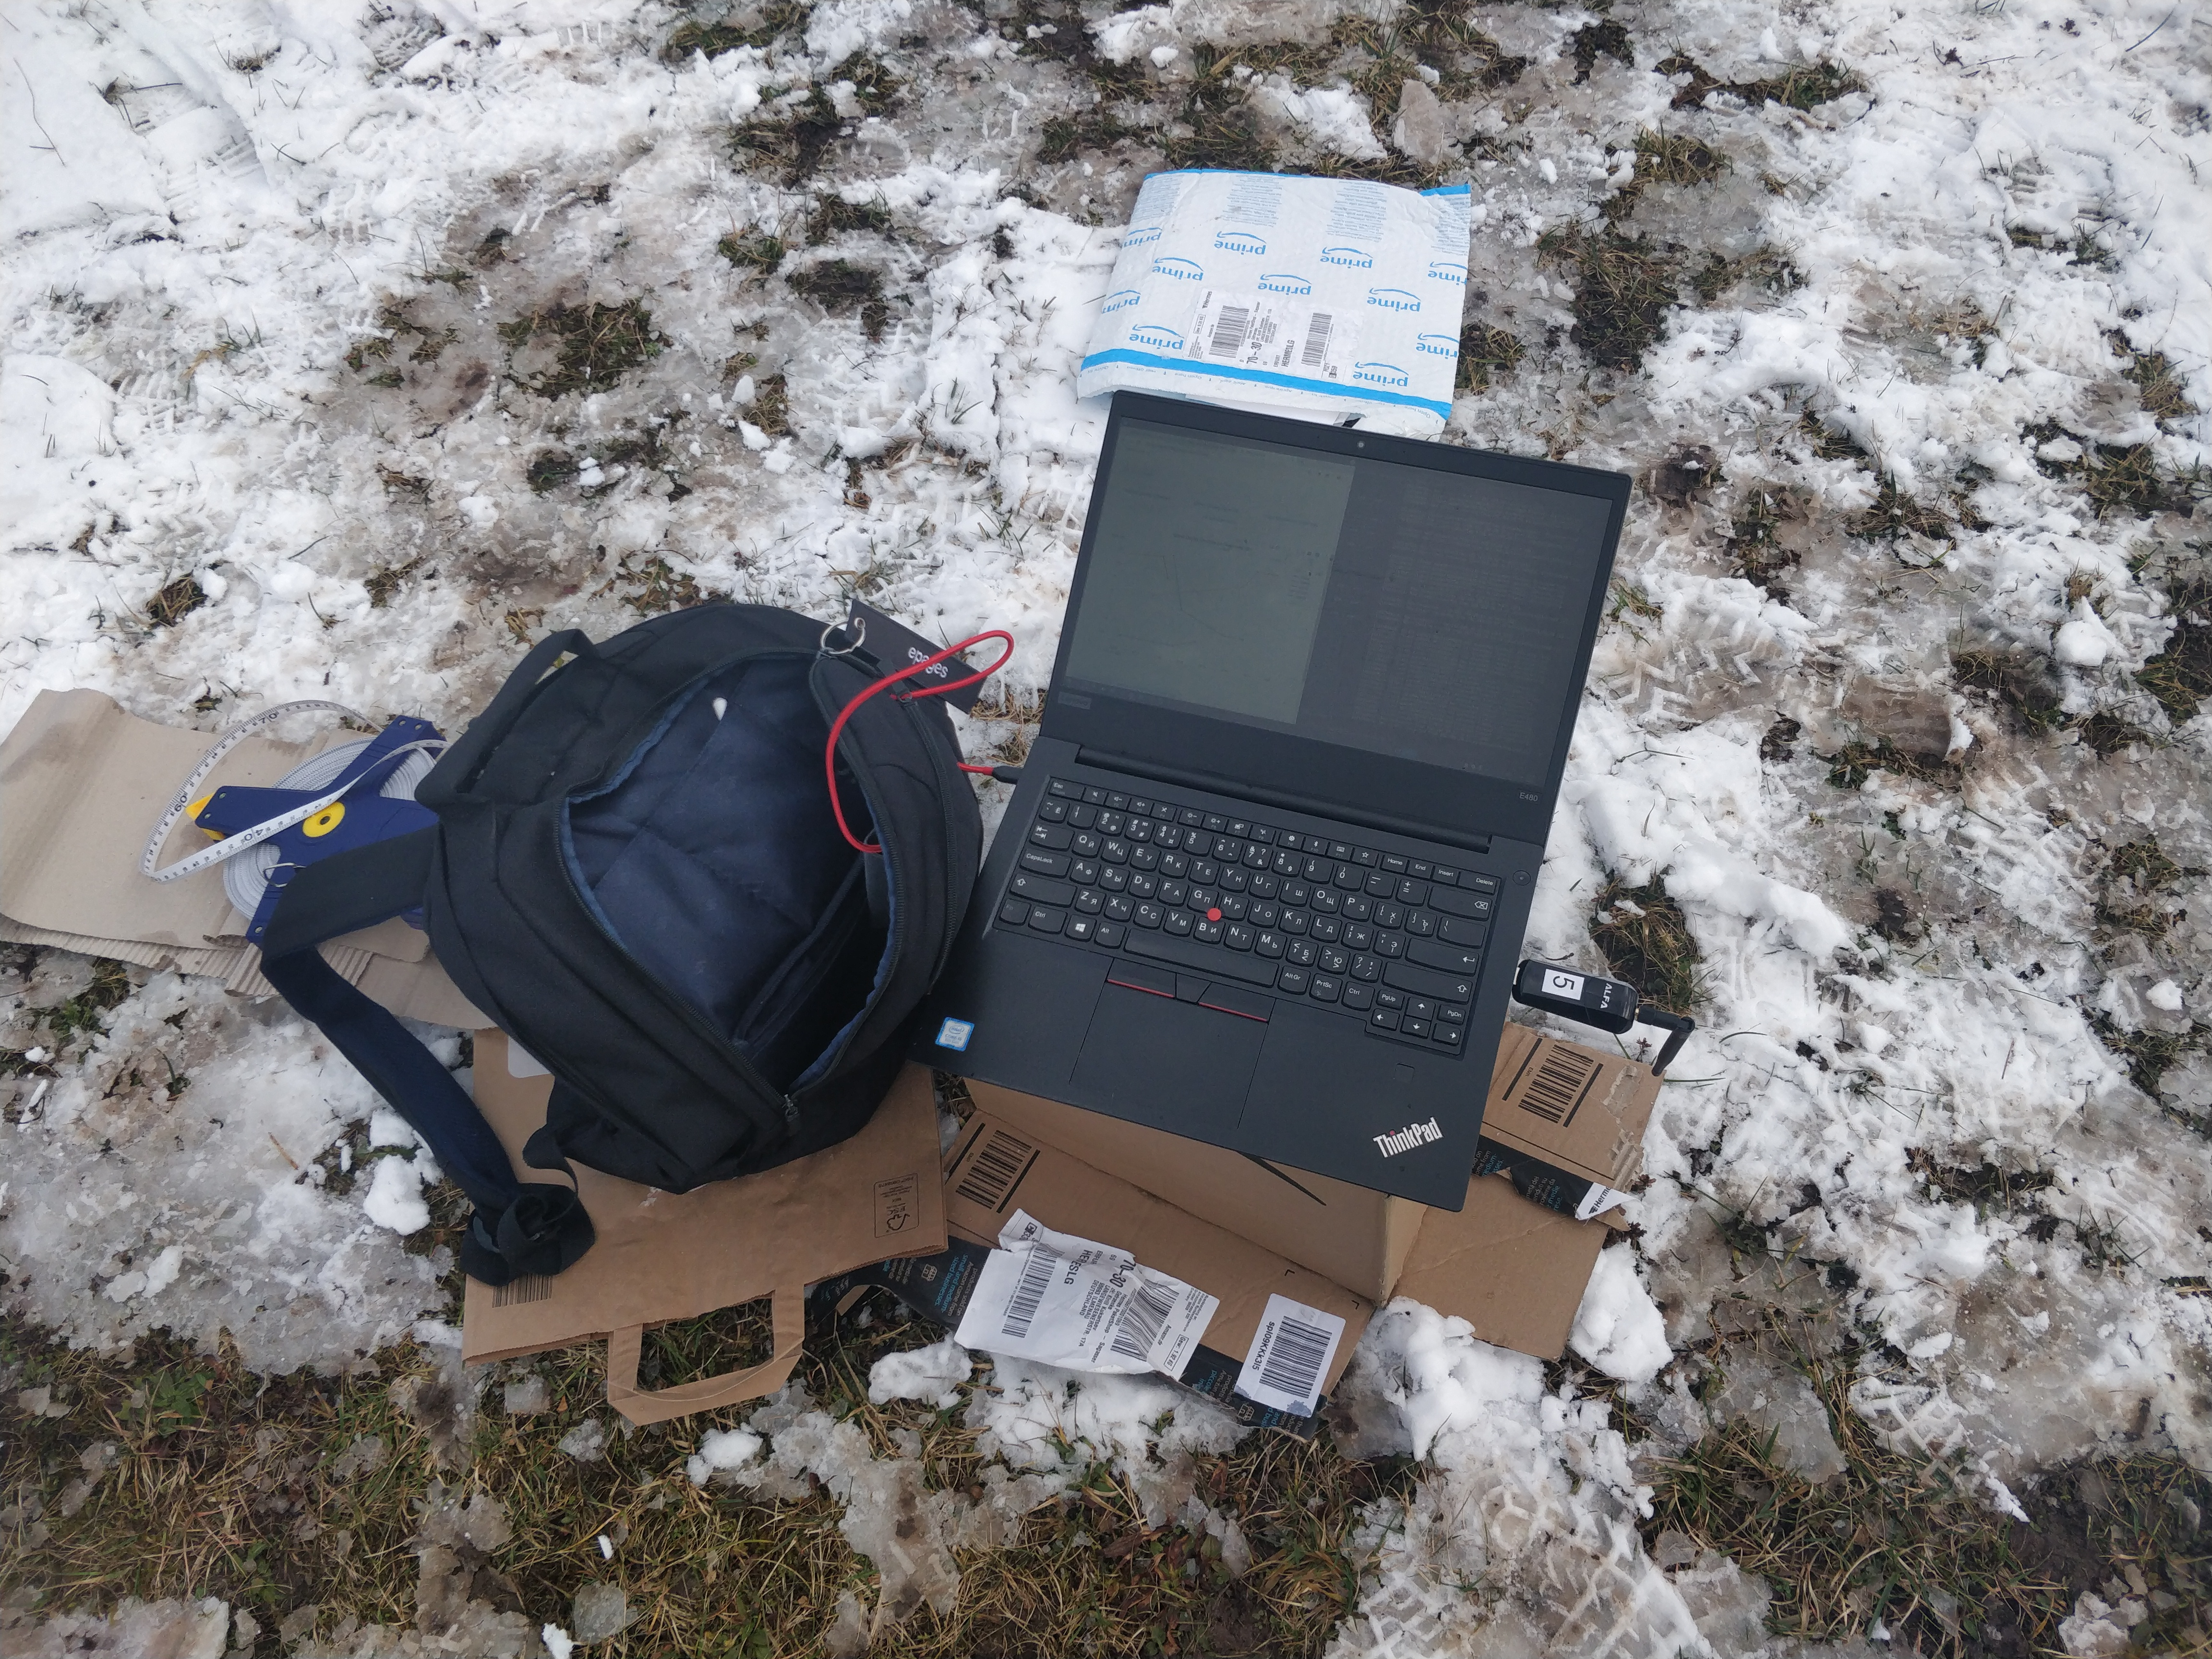
\includegraphics[width=0.6\linewidth,keepaspectratio]{images/experiment_1_cnc.jpg}
	\caption{Layout of \gls{command_n_center} server}
	\label{fig:cnc-position}
\end{figure}

\subsubsection{Case 1}

We started with \hyperref[sub-optimal-layout]{Sub-Optimal case}.

One \gls{ap} functioned correctly - one group of \glspl{ap} connection to one \gls{ap} was made successfully.
Here was a problem with the second group of \glspl{ap} - due to weather conditions we encountered \gls{wifi} module issues of \gls{ap} (the laptop freeze).

After some time of data collection, it was clear the second \gls{ap} was not sending data to \gls{command_n_center} at all, so we decided to locate devices according to \hyperref[near-optimal-layout]{Near-Optimal layout scheme}.

\subsubsection{Case 2}

During \hyperref[near-optimal-layout]{Near-Optimal layout case} we observed increase of \acrshort{rss} level -82 and -84 dBm for the left \gls{ap} to -76 and -80 dBm for the other. Link measurement messages from \glspl{ue} connected to the second \gls{ap} dropped by an unknown reason.

Moreover, \gls{gps_frontend} showed that some \glspl{ue} are close to each other (having approximately the same coordinate), whereas the other 2 were detected much further. It indicates that \glspl{gnss} position measurements are biased.

After, the second \gls{access_point} stopped working at some time. Restart and re-connection of \glspl{ue} did not help to obtain data.


\subsubsection{Case 3}

Because of the problems encountered in the previous case, we decided to stop the experiment and figure out possible solutions.

\subsection{Outcome}

The first trial showed:

\begin{itemize}
	\tightlist
	\item
	Further development and bug fixes of \gls{gps_tracker}  and  \gls{gps_android} required.
	\item
	Tests of placement algorithms can be performed, but due to problems with message sending, we could not prove that the suggested optimal positions would lead to better signal conditions.
\end{itemize}

As a result, we decided to:

\begin{itemize}
	\tightlist
	\item
	Find out and fix the failure reasons for the second \gls{access_point}.
	\item
	Analyze the outliers in \gls{gnss} measured positions.
\end{itemize}

	\subsection{Experiment-2. 22.02.2020}\label{experiment-1.-22.02.2020}

The second attempt took place on 22.02.2020.

This time the aim was to test changes in the system components:

\begin{itemize}
	\tightlist
	\item
	A new way to estimate uplink and downlink speed added in \gls{gps_android} using \gls{ftp} (ability to specify IP address for \gls{cnc} in the app)
	\item
	Logging capabilities in \gls{gps_android}
	\item
	Improvements in \gls{gps_frontend} (the uplink/downlink throughput measurements plot, figures became more informative).
\end{itemize}



The goal is to perform an reduced experiment with 1 \gls{command_n_center}, 1 \gls{ap}, and 3 \glspl{ue} with the same settings from the previous experiment but with modified components.

The second \gls{ap} did not participate because of troubles with \gls{wifi} \gls{access_point} installation drivers (later the update to Debian 11 Testing fixed this problem).

\subsection{Weather conditions}

\begin{itemize}
	\tightlist
	\item
	No precipitation
	\item
	Clear sky
	\item
	No snow
	\item
	Strong winds
\end{itemize}

\subsection{Procedure}

Only \hyperref[near-optimal-layout]{Near-Optimal case} was performed.

To exclude possible bottleneck because of additional wireless bearer between \gls{ap} and \gls{command_n_center}, we tried to measure the direct connection to \texttt{cnc} in short distance (shown in Figure \ref{fig:attempt-2-direct-cnc-connection}).

\begin{figure}[H]
	\centering
	\includegraphics[width=0.7\linewidth,keepaspectratio]{images/experiment_2_overview.jpg}
	\caption{Direct connect to \gls{command_n_center}}
	\label{fig:attempt-2-direct-cnc-connection}
\end{figure}

All \glspl{ue} can connect to \gls{command_n_center} successfully:

\begin{itemize}
	\tightlist
	\item
	deviceId assigned
	\item
	\gls{ue} coordinates displayed
\end{itemize}

During the first half of the experiment, after pressing the `push once' button we received \textbf{uplink/downlink} throughput measurements, however, the values of uplink seemed to be too high \gls{wifi} standard (300 000 kBit/s) compared to downlink (1000-2000 kBit/s).

Later, pressing 'push once' button again did not cause speed re-estimation, the messages from \glspl{ue} did not reach \gls{command_n_center}. The log journal did not contain any error messages. 

\subsection{Outcome}

The second attempt was also not successful. We had not managed to solve the problem in measured data sending. For the next iteration, we proposed to implement some design improvements.

As a result, we decided to:

\begin{itemize}
	\tightlist
	\item
	Add logging capabilities to \glspl{ap}.
	\item
	Implement direct \gls{http} requests and retire \gls{mqtt} broker architecture.
\end{itemize}

	\section{Experiment 3. 07.02.2020}\label{experiment-3.-07.02.2020}

Took place on 27.02.2020

This time the aim was to check how \textbf{2 major updates} of the Android app behave.

The \emph{first} one concerned the usage of HTTP requests instead of MQTT. The reason for it is that all previously detected issues related to MQTT in one way or another.

The \emph{second} update was about complete refactoring of the code. It included not only start following MVVM architectural pattern but also removing of redundant `Connect' button, then real-time interaction with the app coordinates updates the display when `Push continuously' enabled.

\subsection{Procedure}

Due to the bad weather (heavy snowfall), we decided to experiment indoor (Mensa building in TU Ilmenau has enough space inside). 1 CnC, 1 AP, and 3 UEs took part.

All UEs can connect successfully:

\begin{itemize}
\tightlist
\item
  `Push once' button pressed
\item
  deviceId assigned
\item
  UE coordinates displayed
\end{itemize}

\subsection{Tips}

As for `Push continuously', it should be known in advance the
coordinates updated on the display \textbf{only in the case of moving to
some minimal delta} (10 centimeters). This is insured based on GPS
values passed by the Android device.

To make sure the connection is still alive, and the values are transferred, it makes sense to check logging messages in logs/log.txt in UE.

\subsection{Outcome}

To sum up, the system finally started working as expected, and the meaningful set of data is collected, as shown in the following figures.

\begin{figure}[H]
	\centering
	\includegraphics[width=\linewidth,keepaspectratio]{images/experiment_3_1.jpg}
\caption{Movement trajectory of connected phones}
\end{figure}

\begin{figure}[H]
	\centering
	\includegraphics[width=\linewidth,keepaspectratio]{images/experiment_3_2.jpg}
\caption{Signal quality map}
\end{figure}

\begin{figure}[H]
	\centering
	\includegraphics[width=\linewidth,keepaspectratio]{images/experiment_3_3.jpg}
\caption{Signal quality changes}
\end{figure}

	\section{Experiment 4. 03.03.2020}\label{experiment-4.-03.03.2020}

It took place on 03.03.2020. The weather conditions were appropriate for the experiment, although there was raining lightly.

For the fourth trial, we implement sending of measurement messages only with \gls{http} protcol from \gls{ue} to \gls{command_n_center}. 

We aimed to find optimized positions for the \glspl{ue} in three cases (Sub-Optimal, Uniform, Near-Optimal).

We decided to reduce the area layout to 25x25 meters.

We use one smartphone with a special program that can precisely locate the position. Then we placed the phone where \glspl{ue} and \glspl{ap} were, which helped us to find out the initial positions. These coordinates for \glspl{ue} are shown in Table \ref{tab:exp4-initial-coordinates-ues}. We use \texttt{decimal degrees} for coordinates.

\begin{longtable}[]{@{}ll@{}}
	\caption{Initial coordinates for \glspl{ue}}\tabularnewline
	\toprule
	Unique ID & Coordinates\tabularnewline
	\midrule
	\endhead
	f072f812f48ce468 & 50.6823458, 10.94051806\tabularnewline
	eb0b54819c69cf0c & 50.6824625, 10.9403367\tabularnewline
	27349a2cde6592df & 50.6822786, 10.94057\tabularnewline
	51336504999bc1ca & 50.6822861, 10.940590\tabularnewline
	b1c225280d0ed13f & 50.6824403, 10.940343889\tabularnewline
	abb76773bdee4fa0 & 50.6824789, 10.940261944\tabularnewline
	\label{tab:exp4-initial-coordinates-ues}
\end{longtable}


The initial coordinates for \glspl{ap} are shown in Table \ref{tab:exp4-initial-coordinates-aps}.

\begin{longtable}[]{@{}ll@{}}
	\caption{Initial coordinates for \glspl{ap} }\tabularnewline
	\toprule
	AP & Coordinates\tabularnewline
	\midrule
	\endhead
	AP1 & 50.6823778, 10.94054861\tabularnewline
	AP2 & 50.6824281, 10.940313611\tabularnewline
	\bottomrule
	\label{tab:exp4-initial-coordinates-aps}
\end{longtable}

\subsection{Results}

The \gls{http} protocol helped to receive messages reliably, despite there were connection failures, we observed that the farther \gls{ue} is located from \gls{ap}, the less is probable reception of the message. Retransmission of messages implemented in \gls{gps_android} partly mitigated losses.

We found out that network speed measurements were not significant, because there was markedly seen the difference between \texttt{uplink} and \texttt{downlink} speed, uplink tests threw timeout exception in case of the larger distance between a \gls{ue} and a \gls{access_point}, because the communication took longer and the session terminated. 

The experiment is divided into four parts:

\begin{itemize}
	\tightlist
	\item
	Before 11:05 - Sub-Optimal case
	\item
	11:05 - 11:08 - Uniform case
	\item
	11:08 - 11:12 - Near-Optimal case
	\item
	11:12 - 11:15 - Sub-Optimal to compare the suggested positions
\end{itemize}

\subsubsection{Sub-Optimal case}

The first case is the most profitable from the signal quality point of
view. The \glspl{ap} are implicitly located at the same distance from the
connected \glspl{ue}. Signal changes can be seen in Figure \ref{fig:signal-quality-changes-sub-optimal} - despite this case is expected to have the best link parameters, \acrshort{rss} is unstable for \glspl{ue}, possible reason for this - differences in phone generations, e.g. modern phones also include more advanced \gls{wifi} model.

\begin{figure}[H]
	\centering
	\includegraphics[width=0.7\linewidth,keepaspectratio]{images/Exp4_Suboptimal.png}
	\caption{Signal Quality changes in Sub-Optimal case}
	\label{fig:signal-quality-changes-sub-optimal}
\end{figure}

Despite the \glspl{ap} were located close to \glspl{ue}, the \acrshort{rss} level varies noticeably. However, only in this case the speed and signal quality measurement were the most stable among all cases.

\subsubsection{Uniform case}

In this case, the \glspl{ap} are located with equal distance from the \gls{command_n_center}.

\begin{figure}[H]
	\centering
	\includegraphics[width=0.7\linewidth,keepaspectratio]{images/Exp4_Uniform.png}
	\caption{Signal Quality changes in Uniform case}
	\label{fig:signal-quality-changes-uniform-optimal}
\end{figure}

Figure \ref{fig:signal-quality-changes-uniform-optimal} depict \acrshort{rss} changes in Uniform case. Link measurement is more steady and keeps on the same level for the majority of \gls{ue}, however, we encountered speed test failed.

\subsubsection{Near-optimal case}

The third case simulates the situation where the \glspl{ap} are placed
uniformly far from centers of \glspl{ue} clusters.

Figure \ref{fig:signal-quality-changes-near-optimal} demostrates that measured \acrshort{rss} lower than in Uniform case because of larger distance between \glspl{ap} and \glspl{ue} approximately on 10-15 dBm.

\begin{figure}[H]
	\centering
	\includegraphics[width=0.7\linewidth,keepaspectratio]{images/Exp4_Near_Optimal.png}
	\caption{Signal Quality changes in Near-optimal case}
	\label{fig:signal-quality-changes-near-optimal}
\end{figure}

\subsubsection{Comparison between real coordinates in Sub-Optimal case layout and real positions
	positions}

To check the validity, we place the \glspl{ap} in a Sub-Optimal case position. Figure \ref{fig:ues-positions-for-optimization} represents the most recent positions  of \glspl{ue} as input data used for optimization tasks. The exact coordinates are presented in Table \ref{tab:exp4-sub-optimal-last-received-coordinates-ues}.

\begin{longtable}[]{@{}ll@{}}
	\caption{The last received coordinates for \glspl{ue} by \gls{gps_android}}\tabularnewline
	\toprule
	Unique ID & Coordinates\tabularnewline
	\midrule
	\endhead
	27349a2cde6592df* & 50.68206, 10.94044\tabularnewline
	51336504999bc1ca* & 50.68206, 10.94044\tabularnewline
	f072f812f48ce468* & 50.6823, 10.9406\tabularnewline
	b1c225280d0ed13f* & 50.68243, 10.94035\tabularnewline
	abb76773bdee4fa0* & 50.6823, 10.93987\tabularnewline
	eb0b54819c69cf0c* & 50.68253, 10.93984\tabularnewline
	\bottomrule
	\label{tab:exp4-sub-optimal-last-received-coordinates-ues}
\end{longtable}

\begin{figure}[H]
	\centering
	\includegraphics[width=0.5\linewidth,keepaspectratio]{images/Exp4_UEs_Location_to_optimize.png}
	\caption{The \glspl{ue} coordinates used to optimize \glspl{ap} positions}
	\label{fig:ues-positions-for-optimization}
\end{figure}

The coordinates for \textbf{27349a2cde6592df} and
\textbf{51336504999bc1ca} overlap.

The most recent received coordinates for \glspl{ue} used to schedule an optimization task with the following parameters:

\begin{itemize}
	\tightlist
	\item
	Number of clusters: 2
	\item
	Estimation method: ``clustering''
\end{itemize}

The ``simplex'' method against two clusters is not possible. Instead we use 'clustering' method which uses K-means clusterization algorithm. Figure \ref{fig:ues-positions-and-suggested-optimal-positions-for-uavs} demonstrate positions for \glspl{ue} as blue dots and suggested coordinates for two \glspl{ap} as black box.

\begin{figure}[H]
	\centering
	\includegraphics[width=0.5\linewidth,keepaspectratio]{images/Expt4_Estimated UAVs_locations.png}
	\caption{Result of optimization task to obtain optimal positions for \glspl{ap}}
	\label{fig:ues-positions-and-suggested-optimal-positions-for-uavs}
\end{figure}

The suggested optimal coordinates for \glspl{ap} are shown in Table \ref{tab:optimal-coordinates}.

\begin{longtable}[]{@{}lll@{}}
	\caption{Suggested optimal positions for \glspl{uav} }\tabularnewline
	\toprule
	AP & Real coordinates & Suggested coordinates\tabularnewline
	\midrule
	\endhead
	AP1 & 50.6823778, 10.94054861 & 50.68221, 10.94046\tabularnewline
	AP2 & 50.6824281, 10.940313611 & 50.68245, 10.93986\tabularnewline
	\bottomrule
	\label{tab:optimal-coordinates}
\end{longtable}

Figure \ref{fig:optimized-coordinates-on-logical-map} shows on the map real and suggested optimal coordinates for \gls{ap}. These new positions can drop out connected clients due to large distance because at this space connection became unstable, their error rate is higher.

This figure contains four types of elements:

\begin{enumerate}
	\item Green circles - represent initial coordinates for \glspl{ue}.
	
	\item Red circles - represent coordinates for \glspl{ue} received by \gls{gps_android}.
	
	\item Yellow tags - represent initial coordinates for \glspl{ap}.
	
	\item Blue tags - represent suggested optimal coordinates for \glspl{ap}.
	
\end{enumerate}

\begin{figure}[H]
	\centering
	\includegraphics[width=\linewidth,keepaspectratio]{images/Expt4_Result_of_optimization_map_with_names.png}
	\caption{Original and Optimized Coordinates: A map with tags.}
	\label{fig:optimized-coordinates-on-logical-map}
\end{figure}

Distance between real and suggested positions for AP1 is 32m and 20m for AP2 accordingly. We find out two possible reasons for this difference:

\begin{enumerate}
	\item Fragmentation of used \gls{android} phones - in the experiment we used various gadgets running different \gls{os} version. They present several generations of \gls{android} evolution. The older generations can have less accurate \gls{gnss} module, therefore provide a wrong position estimate.
	\item Location provider optimization in \gls{gps_android} - \gls{gps_android} was designed  to choose between network-assisted and \acrshort{gps}-assisted location estimation. The exact option depends on what provider has better connection status. First, it tries to set up \acrshort{gps} provider, if it fails, the phone fallback to network-provided location estimation which is less accurate.
\end{enumerate}


Figure \ref{fig:optimized-coordinates-satellite-map} depict these coordinates on the map from a satellite point of view.

\begin{figure}[H]
	\centering
	\includegraphics[width=0.5\linewidth,keepaspectratio]{images/Expt4_Result_of_optimization_sattelite.png}
	\caption{Original and Optimized Coordinates for \glspl{uav}: A map from satellites.}
	\label{fig:optimized-coordinates-satellite-map}
\end{figure}

``Clustering'' algorithm performs simple K-means cluster calculation
based on \gls{gnss} coordinates for \glspl{ue}. The result provides insights about that layout optimization algorithms relying solely on the coordinate input data can result in a biased solution.

\subsection{Outcome}

Finally, we have managed to test the framework and estimate an optimized position for \glspl{uav} which were represented by \gls{wifi} access points. The results showed that the framework match requirements, however, should be redesigned and evaluated on updated data.

	\clearpage
\section{Final Results}\label{final-results}

We have completed 4 experimental attempts. We encountered problems each
attempt, mostly they cover:

\begin{itemize}
\tightlist
\item
  Wi-Fi connection: radio link may suffer serious collisions that drop
  up data transmission.
\item
  Complicated architecture: the initial proposed design is
  quite sophisticated, but it does not match the given functional
  requirement. Further, we figured out a possible simplified solution
  that gave us an opportunity to run experiments correctly, however,
  there are still gaps to fill in.
\item
  Optimization algorithms: higher accuracy requires additional data to
  supply and more advanced algorithms to perform. Even so, there should
  be a strict evaluation of the results they produce if that is correct.
\end{itemize}

Despite these problems, we can conclude that the developed framework can
be applied for performing UAVs layout optimization, the current version
has enough capabilities to provide access to investigate and analyze the
measured data. The algorithms included in the current version of the
framework have restrictions, simplified and produce biased results, but
the contrary has an ability to be highly modified to obtain more
reliable results. The extensibility of the platform gives the
opportunity to extend the current set of optimization algorithms in a
simple way.

	
	\newpage
	
	\printglossary
	\clearpage
	
	\printglossary[type=\acronymtype]
	
	\clearpage
	
	\printbibliography[heading=bibintoc,title={References}]
	
	\clearpage
	
	\begin{appendix}
		\listoffigures
		\listoftables
	\end{appendix}
	

	
\end{document}